\section{Acceptance and Efficiency Correction}
\label{sec:AccXEff}

% A is the fiducial and kinematic acceptance,
% is the selection efficiency for events in the acceptance,

The unfolded $P_T^{\gamma}$ spectrum needs to undergo several corrections in order to obtain the true $P_T^{\gamma}$ spectrum in the chosen phase space: the selection efficiency, the reconstruction efficiency, and the acceptance corrections. The total background-subtracted yield needs to undergo these corrections as well. The nature of these corrections and the methods of their application are explained below.

The selection requirements in the $W\gamma$ measurement are stricter than the phase space requirements for the cross section measurement (Ch.~\ref{sec:AN_WgMeas}), thus, during the selection procedure, we discard a large number of signal events that are within the phase space. The ratio between the number of selected signal events and the number of signal events reconstructed within the phase space is called a ``selection efficiency''. 

In addition to the event loss due to the selection requirements, a certain number of events are truly within our phase space but are reconstructed outside of the phase space or are not reconstructed at all and vice versa. A ratio between the number of signal events that are reconstructed within our phase space and the number of events that truly appear within our phase space is called a ``reconstruction efficiency''. The procedure of the detector resolution unfolding (Ch.~\ref{sec:Unfolding}) takes care of this effect for $P_T^{\gamma}$ phase space requirement in the $P_T^{\gamma}$ yields, however effects of other phase space requirements for both $P_T^{\gamma}$ and total yields and the $P_T^{\gamma}$ requirement for the total yield still need to be taken into account.

Finally, certain events that are truly within the phase space may not be caught by the detector due to the detector acceptance restrictions. Examples of such events include events with final state photons or electrons that go into the gap between the EB and EE, with corresponding 1.44$<|\eta^{\gamma,e}|<$1.56. A ratio between the number of events truly reconstructed within the phase space, and the number of events that are also registered by the detector is called ``acceptance''.  

To correct our selected, background-subtracted, unfolded yields from Tab.~\ref{tab:unf_results_MUON_WGamma}-\ref{tab:unf_results_ELECTRON_WGamma} for these effects, we introduce a correction $A \times \epsilon$ that accumulates all three effects described above. The correction is estimated using the signal MC sample, separately for the total yield and $P_T^{\gamma}$ yields. 

The numerator $N^{A\epsilon}$ for the correction of the total yield is determined as the number of selected events in the signal MC with the PU weight applied. The numerator $N^{A\epsilon}_i$ for the correction of the  $P_T^{\gamma}$ yields is determined as selected signal MC yields with the PU weight applied in $P_T^{\gamma(gen)}$ bins at the gen-level. Index $i$ stands for $P_T^{\gamma}$ bins.

The denominator $D^{A\epsilon}$ of the $A \times \epsilon$ correction is determined as the number of events that are within the phase space based on their kinematic parameters. For the correction $(A \times \epsilon)_i$ of the $P_T^{\gamma}$ yields, the numbers $D^{A\epsilon}_{i}$ are determined separately for each $P_T^\gamma$ bin.  

The $A \times \epsilon$ correction is determined then as $A \times \epsilon = N^{A\epsilon}/D^{A\epsilon}$ for the total yield and as $(A \times \epsilon)_i = N^{A\epsilon}_i/{D^{A\epsilon}_i}$ for the $P_T^{\gamma}$ yields where index $i$ stands for a $P_T^{\gamma}$ bin. The $A \times \epsilon$ for the total yield are~0.2891$\pm$0.0006 for the muon channel and~0.1229$\pm$0.0004 for the electron channel. The uncertainties are determined by the statistical power of the $W\gamma$ MC sample. The values of the $(A \times \epsilon)_i$ correction for the $P_T^{\gamma}$ yields are plotted in Fig.~\ref{fig:accXeff_Wg}.

\begin{figure}[htb]
  \begin{center}
     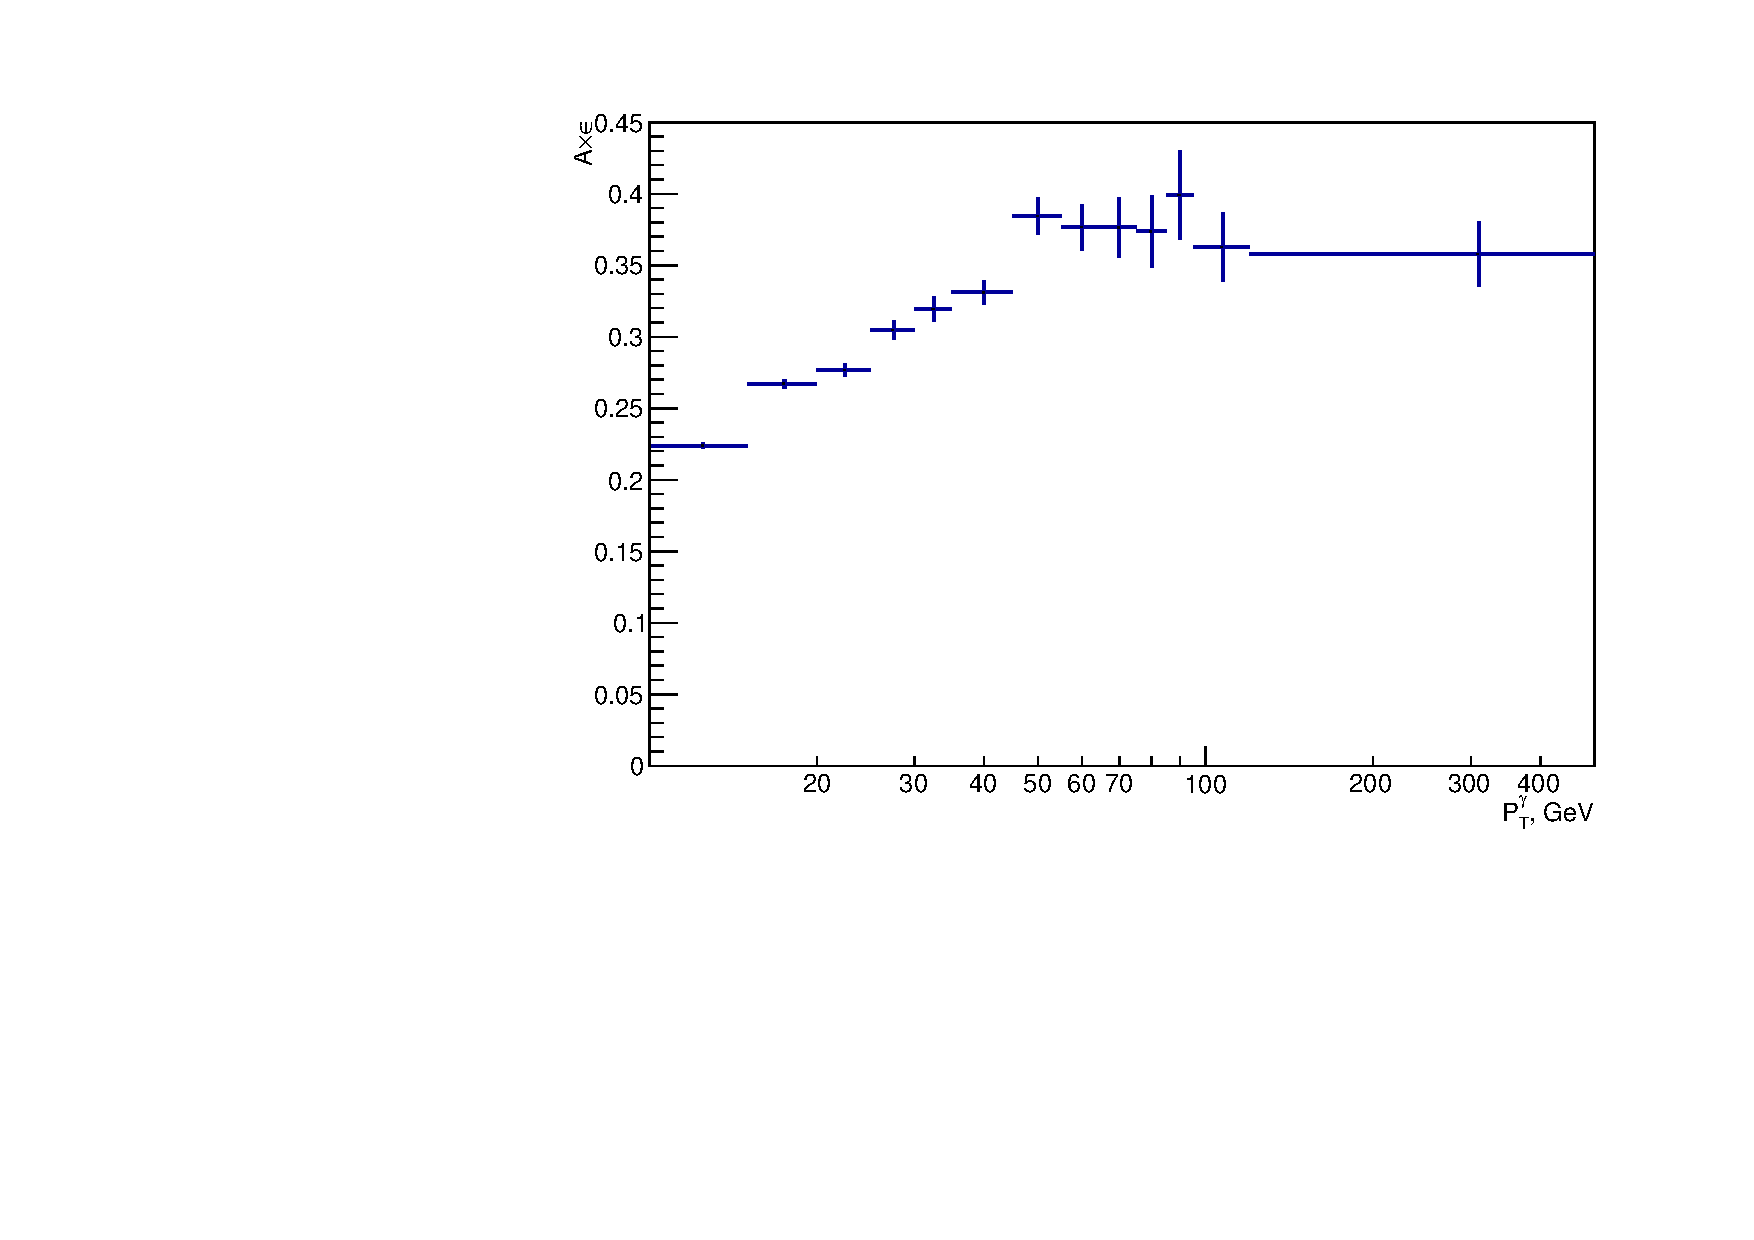
\includegraphics[width=0.48\textwidth]{../figs/figs_v11/MUON_WGamma/Constants/C_accXeff_MUON_WGamma.pdf}  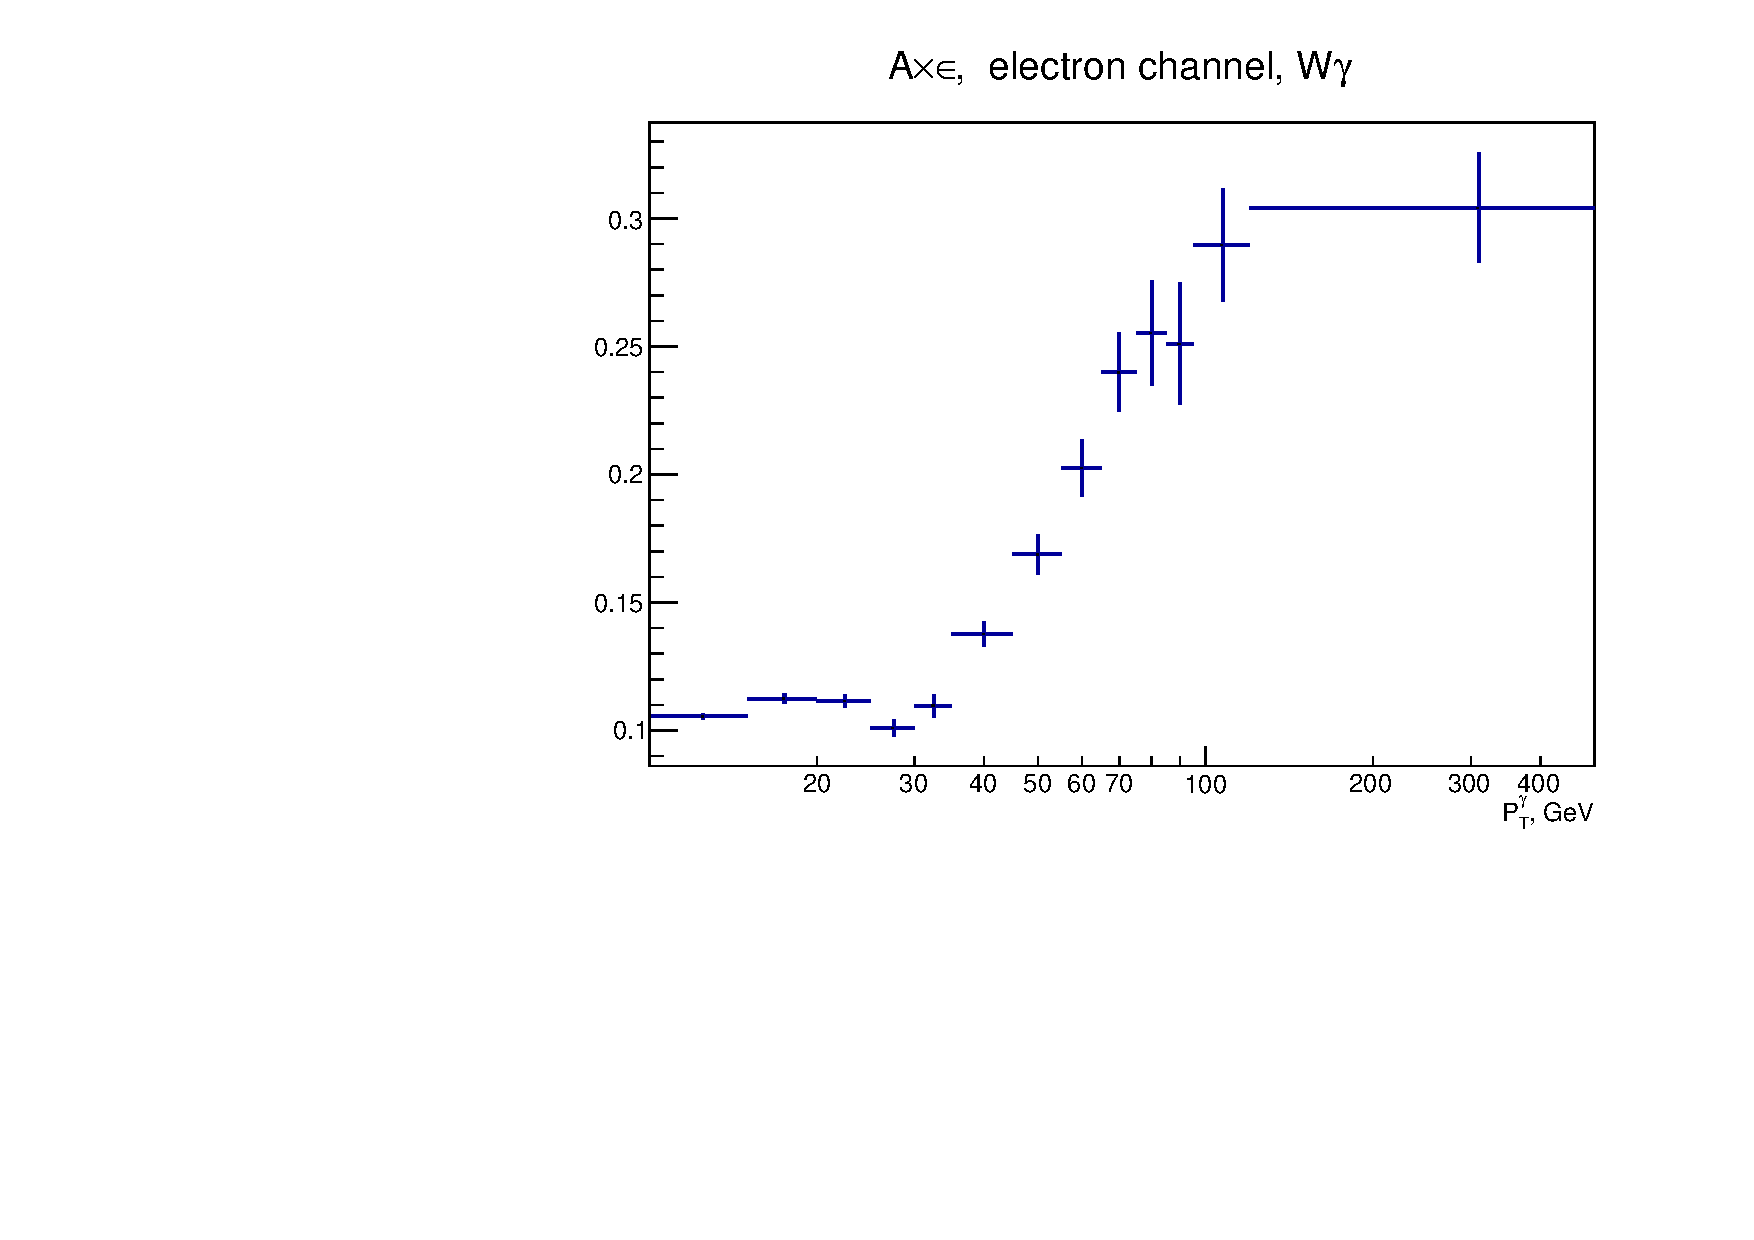
\includegraphics[width=0.48\textwidth]{../figs/figs_v11/ELECTRON_WGamma/Constants/C_accXeff_ELECTRON_WGamma.pdf}
 \caption{$A\times\epsilon$ corrections in the muon (left) and electron (right) channels. Plots are produced with $W\gamma$ MC sample at $\sqrt{s}=$8~TeV. }
  \label{fig:accXeff_Wg}
  \end{center}
\end{figure}

%To determine whether the event within the phase space or not, the following algorithm was used:
%\begin{itemize}
%   \item find a muon/electron which has a W boson as a mother particle
%   \item add 4-momenta of the dressing photons to the 4-momentum of the muon/electron; dressing photons as defined as photons that have $P_T>0.5$ GeV and have $\Delta R(lepton,photon)<0.1$
 %  \item find a final state photon which corresponds to FSR, ISR or TGC; exclude dressing photons from the consideration
 %  \item using 4-momentum of the photon and the adjusted 4-momentum of the lepton, determine whether the event is within the phase space or not
%\end{itemize}

